\chapter{Aspectos conceituais}
\label{CAP2}


A seguir serão explicados os conceitos fundamentais que possibilitam a execução deste trabalho. 


\section{Efeito Estroboscópico}

O efeito estroboscópico será a base de funcionamento do projeto. Descoberto na década de 1830, esse fenômeno consiste no uso de diferentes técnicas para a captura de um movimento contínuo ou cíclico com um taxa de amostragem feita de tal maneira que o  movimento aparente é nulo.

Neste projeto, será usado um variação especifico do fenômeno conhecida como Efeito da Roda-de-Carroça (\textit{Wagon-wheel effect}) \cite{tessive}. O nome é originado dos filmes de faroeste em que as rodas das carroças pareciam se mover no sentido oposto ao que era esperado\cite{wagon_wheel}.

O Efeito da Roda-de-Carroça  acontece quando a taxa de quadros por segundo na câmera é um múltiplo do período de rotação de um objeto, fazendo-o parecer parado, se movimentando devagar ou num sentido inesperado. 

O efeito pode ter vários usos práticos, como para a calibração da velocidade de um disco de vinil ou para maquinário pesado.

As figuras \ref{fig:vinil} e \ref{fig:helicopter} ilustram o fenômeno físico em questão.

\begin{figure}[H]
    \centering
    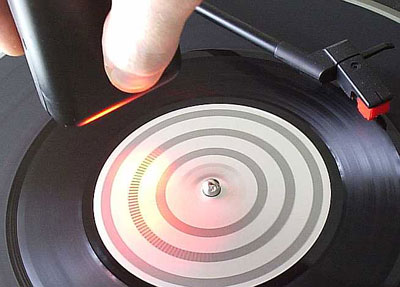
\includegraphics[width=0.8\textwidth,angle=0]{figures/strobe_3.jpg}
    \caption{Demonstração do efeito estroboscópico sobre um disco de vinil.}
    \label{fig:vinil}
\end{figure}

\begin{figure}[H]
    \centering
    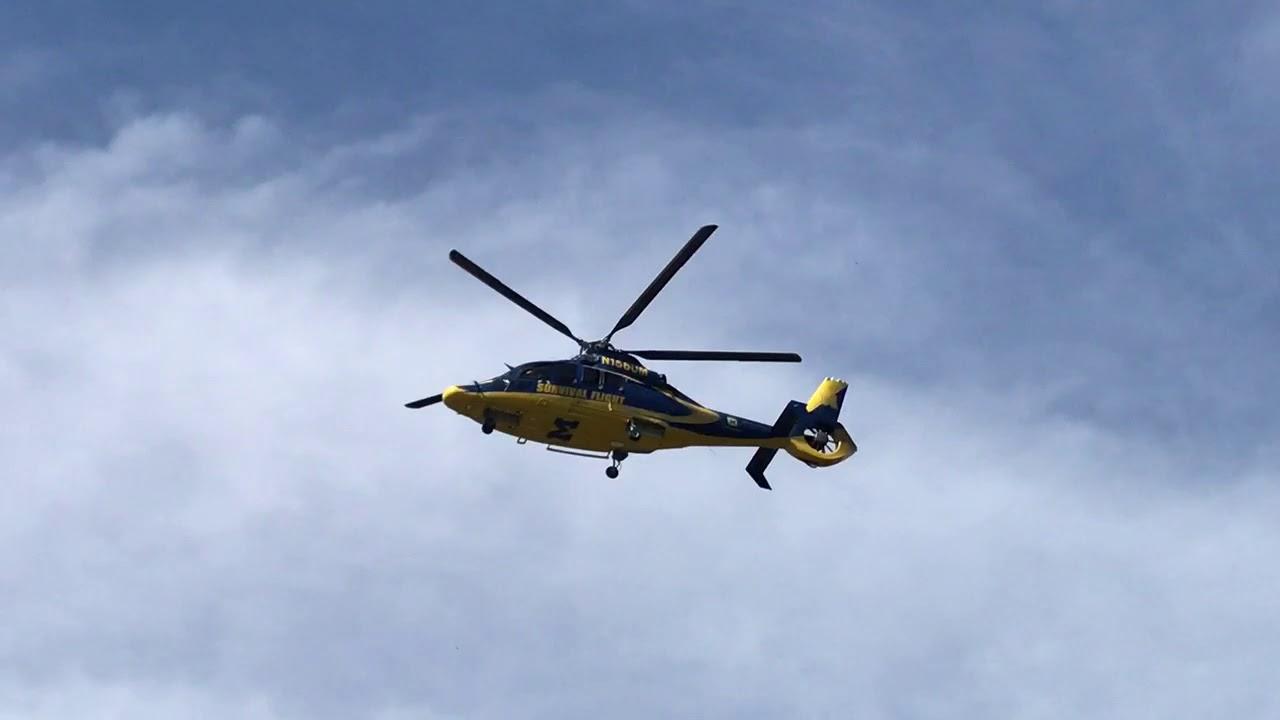
\includegraphics[width=0.8\textwidth,angle=0]{figures/helicoptero_parado.jpg}
    \caption{O rotor do helicóptero parece parado graças ao efeito roda-de-carroça.}
    \label{fig:helicopter}
\end{figure}
\pagebreak

\section{\textit{Motion Blur}}

\textit{Motion Blur} (borrar imagem em movimento), ocorre quando um objeto se movimenta durante o período de exposição de uma fotografia. 

O \textit{blur} é benéfico em muitas situações, pode fazer o movimento rápido de um objeto parecer mais suave, mas quando uma câmera se move existem dois problemas: a imagem pode ficar completamente borrada e, em câmeras mais simples como as de celulares, o \textit{blur} pode confundir o sistema de foco automático, gerando uma imagem borrada, mesmo com exposições baixas. 

A imagem \ref{fig:blur} ilustra o que seria uma imagem borrada devido a tremer demais a câmera durante uma foto.

\begin{figure}[H]
    \centering
    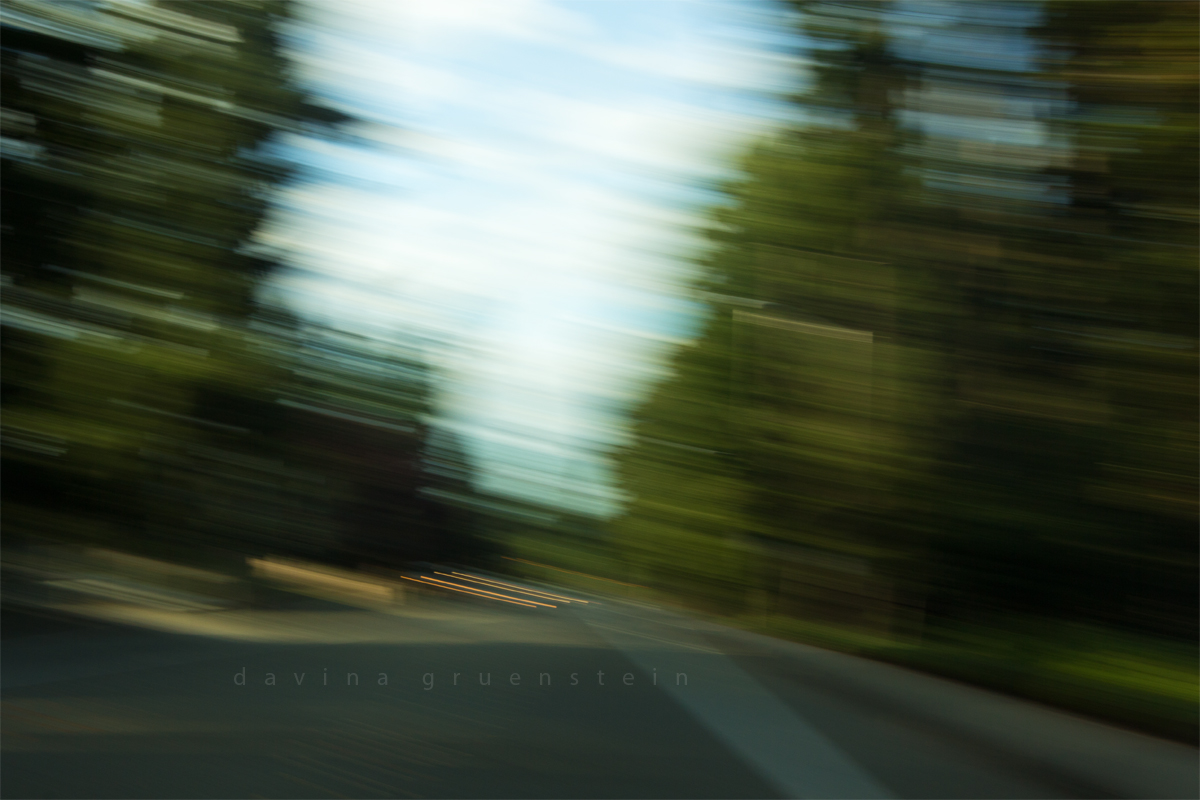
\includegraphics[width=0.9\textwidth,angle=0]{figures/motion-blur3.jpg}
    \caption{Imagem borrada devido ao motion blur. Imagem de: Davina Gruenstein}
    \label{fig:blur}
\end{figure}